\documentclass[10pt]{beamer}
\usetheme[
%%% option passed to the outer theme
%    progressstyle=fixedCircCnt,   % fixedCircCnt, movingCircCnt (moving is deault)
  ]{Feather}
  
% If you want to change the colors of the various elements in the theme, edit and uncomment the following lines

% Change the bar colors:
%\setbeamercolor{Feather}{fg=red!20,bg=red}

% Change the color of the structural elements:
%\setbeamercolor{structure}{fg=red}

% Change the frame title text color:
%\setbeamercolor{frametitle}{fg=blue}

% Change the normal text color background:
%\setbeamercolor{normal text}{fg=black,bg=gray!10}

%-------------------------------------------------------
% INCLUDE PACKAGES
%-------------------------------------------------------

\usepackage[utf8]{inputenc}
\usepackage[english]{babel}
\usepackage[T1]{fontenc}
\usepackage{helvet}
\usepackage{xcolor}


%-------------------------------------------------------
% DEFFINING AND REDEFINING COMMANDS
%-------------------------------------------------------

% colored hyperlinks
\newcommand{\chref}[2]{
  \href{#1}{{\usebeamercolor[bg]{Feather}#2}}
}
\providecommand{\tightlist}{%
  \setlength{\itemsep}{0pt}\setlength{\parskip}{0pt}}

\newcommand\ytl[2]{
\parbox[b]{8em}{\hfill{\color{gray}\bfseries\sffamily #1}~~}\makebox[0pt][c]{$\bullet$}\vrule\quad \parbox[c]{7cm}{\vspace{7pt}\color{red!40!black!80}\raggedright\sffamily #2\\[7pt]}\\[-3pt]}

%-------------------------------------------------------
% INFORMATION IN THE TITLE PAGE
%-------------------------------------------------------

\title[i2b2 impemented over SMART-on-FHIR] % [] is optional - is placed on the bottom of the sidebar on every slide
{ % is placed on the title page
      \textbf{i2b2 impemented over SMART-on-FHIR}
}


\author[AP--HP]
{       Mike Mendis  \& Nicolas Paris
}

\institute[AP--HP]
{

\includegraphics[height=.1\textheight]{images/partners.png}

\includegraphics[height=.1\textheight]{images/aphp.jpg}
~\\
      \ttfamily{Partners} (Shawn Murphy) \\
	\ttfamily{AP-HP} (Christel Daniel) \\
  
  %there must be an empty line above this line - otherwise some unwanted space is added between the university and the country (I do not know why;( )
}

\date{\today}

%-------------------------------------------------------
% THE BODY OF THE PRESENTATION
%-------------------------------------------------------

\begin{document}

%-------------------------------------------------------
% THE TITLEPAGE
%-------------------------------------------------------

{\1% % this is the name of the PDF file for the background
\begin{frame}[plain,noframenumbering] % the plain option removes the header from the title page, noframenumbering removes the numbering of this frame only
  \titlepage % call the title page information from above
\end{frame}}
%
%
%\begin{frame}{Content}{}
%	\tableofcontents[hideallsubsections]
%\end{frame}

%-------------------------------------------------------
\section{Context}
\begin{frame}{Context}{EHR federation}

\begin{itemize}
\item i2b2 has more than 200 implementations over the world
\item Multicenter research produces more powerfull results
\item Federation tools such Shrine, Insite, Trinetx federate multiple i2b2 instances
\end{itemize}
$\rightarrow$ What about institutions without i2b2 ?

\end{frame}

%-------------------------------------------------------
\section{Problem}
\begin{frame}{Problem}{Install i2b2 everywhere ?}

\begin{block}{Data Velocity}
\begin{itemize}
	\item[] ETL processes are time/space/humans consuming
	\item[] i2b2 needs a dedicated informatic team
\end{itemize}
\end{block}

\begin{block}{Data Variety}
\begin{itemize}
	\item[] Terminology Mapping tools in their infancy
	\item[] Big Data i2b2 star schema cannot handle
\end{itemize}
\end{block}

\begin{block}{Data Volume}
\begin{itemize}
	\item[] Big Data i2b2 star schema cannot handle
	\item[] Dedicated technology

\end{itemize}
\end{block}

\end{frame}

%-------------------------------------------------------
\section{Solution}
\begin{frame}{Solution}{SMART-on-FHIR}

\begin{itemize}
\item FHIR specifies how EHR should share data
\item FHIR specifies both a \emph{Search} \& a \emph{Terminology Mapping} API
\item EHR vendors are more \& more FHIR conformant
\item SMART-on-FHIR specifies how Apps should consume data
\end{itemize}
$\rightarrow$ Let's i2b2 be a SMART-on-FHIR app !
\end{frame}

%-------------------------------------------------------
\section{Methods}
\begin{frame}{Methods}{i2b2-FHIR}

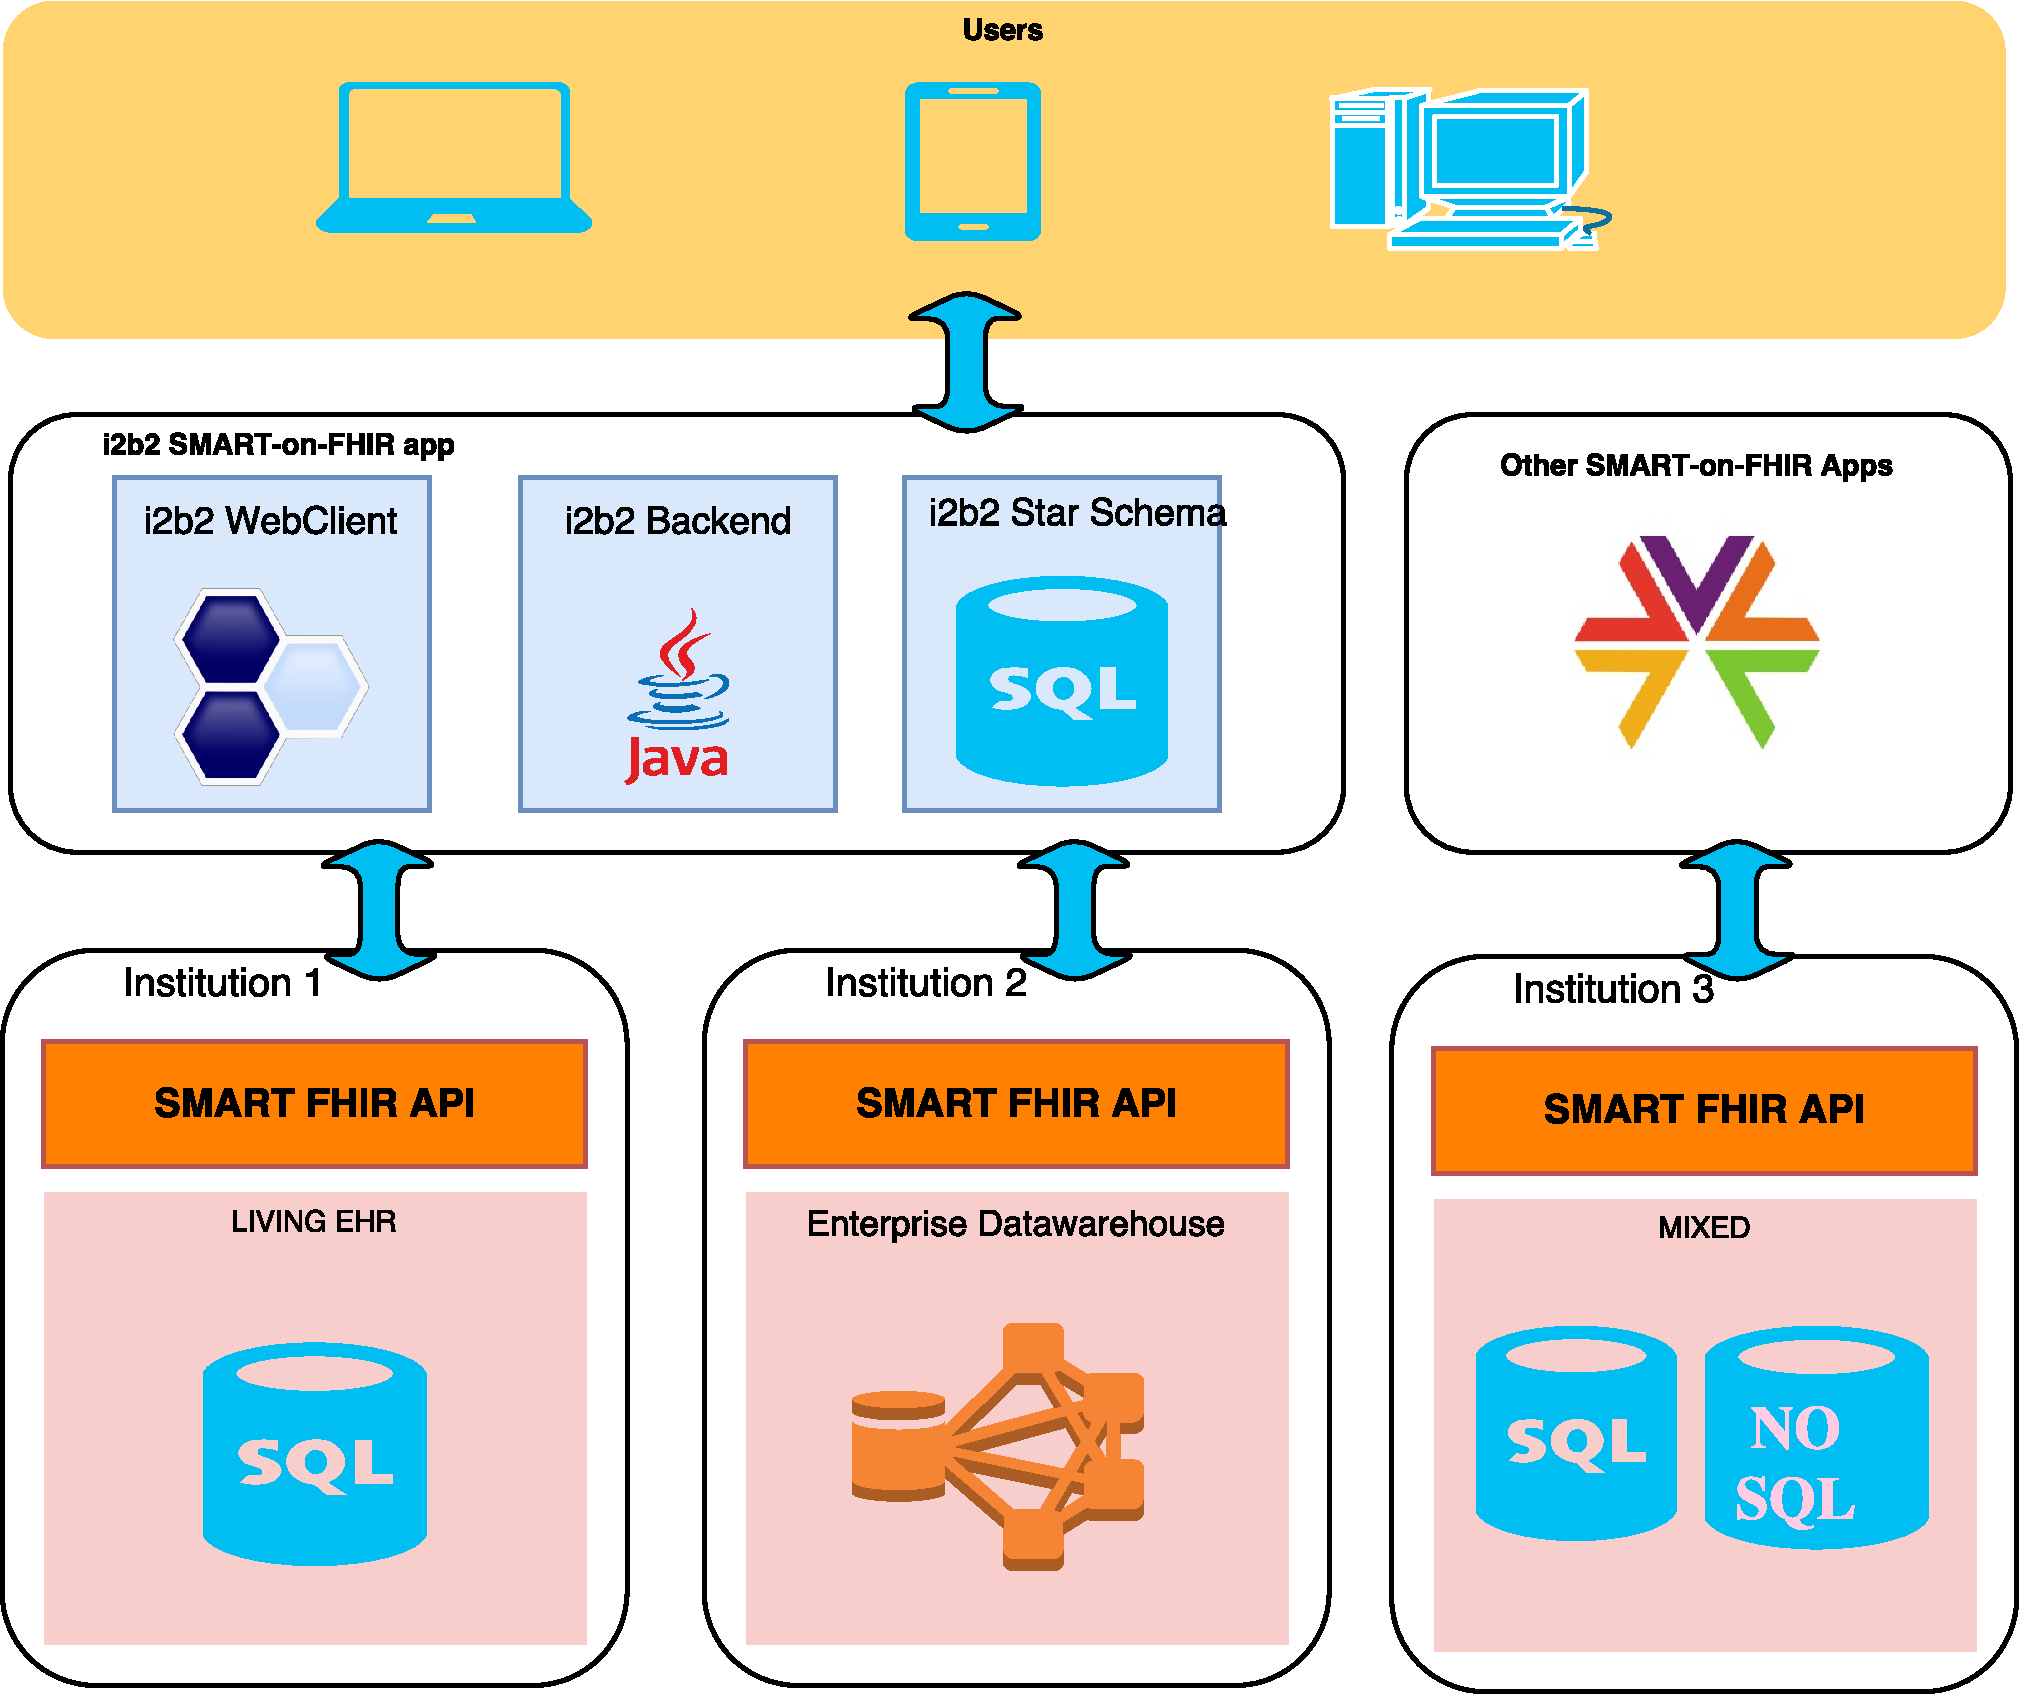
\includegraphics[height=.8\textheight]{images/overall.pdf}
% * <niparisco@gmail.com> 16:56:17 03 Oct 2017 UTC+0200:
% will improve that diagram
\end{frame}

%-------------------------------------------------------
\section{Results}
\begin{frame}{Results}{Implementation}
	Change made to CRC cell
\begin{itemize}
\item New	pm\_cell\_data entry	to	point	to	URL of FHIR
\item By	using	the	project\_path can	configure	to	use	 different	FHIR	API	for	different	projects
\item Easy	to	change	without	restarting	i2b2
\item Limited	to	one	FHIR	API	per	project
\end{itemize}
~
\\
	Change made to PM cell
\begin{itemize}
\item New class written	that extends	Panel Items
\item Any ontology item that begins with \\FHIR is sent to the new class
\item The	Item	Code,	constraint	value	and	date	contraints are	sent	to	the	FHIR	API
\item \ldots
\end{itemize}
\end{frame}

%-------------------------------------------------------
\section{Results}
\begin{frame}{Results}{Screenshot}
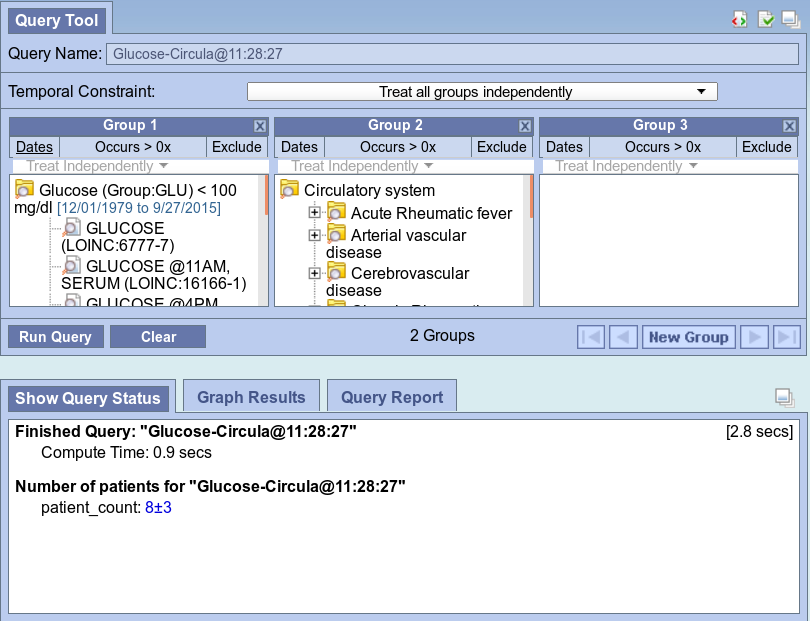
\includegraphics[height=.7\textheight]{images/demo.png}

	$\rightarrow$ Mixed Query is Working (star schema/FHIR endpoint)
\end{frame}
%-------------------------------------------------------
\section{Results}
\begin{frame}{Results}{Benchmarks}
 \begin{columns}[T,onlytextwidth]
        \begin{column}{.6\textwidth}
            \begin{onlyenv}
                \begin{minipage}{\textwidth}
                    \begin{figure}
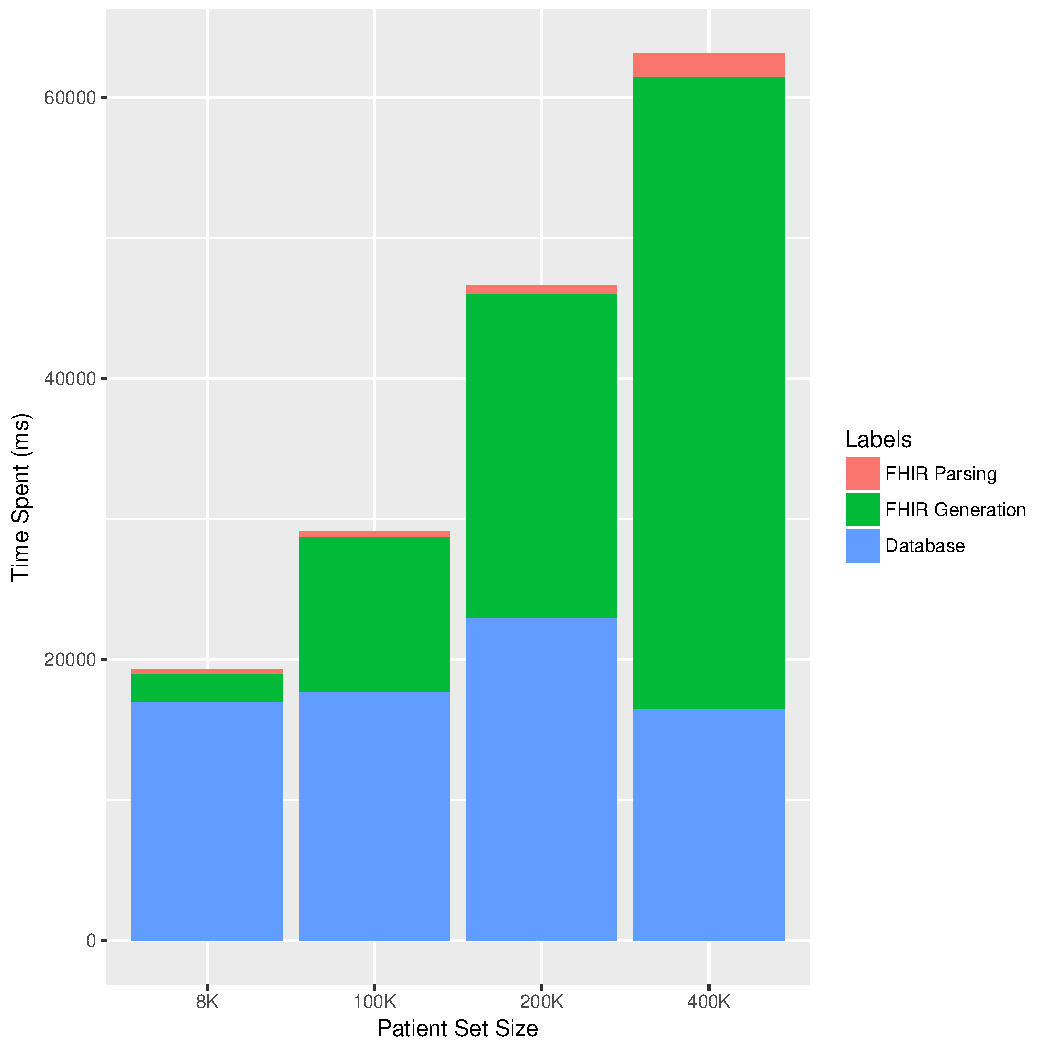
\includegraphics[height=.7\textheight]{images/graph1.pdf}
                    \end{figure}
                \end{minipage}
            \end{onlyenv}
        \end{column}
        \begin{column}{.4\textwidth}
            \begin{onlyenv}
                \begin{minipage}{\textwidth}
			~\\
			~\\
			~\\
	5B physiological table
	\begin{itemize}
		\item FHIR generation step bottlneck
		\item under the minute
		\item sub-linear performances
	\end{itemize}
	$\rightarrow$ Bridging the gap (i2b2 / big-data platforms)
                \end{minipage}
            \end{onlyenv}
        \end{column}
    \end{columns} 

\end{frame}

%-------------------------------------------------------
\section{Discussion}
\begin{frame}{Discussion}{}
Work done:
\begin{itemize}
\item Ontology Model
\item Querying FHIR API
\item Mixed star schema \& FHIR API \& No-SQL DBs
\end{itemize}
~
	\\
	Roadmap:
\begin{itemize}
\item Oauth2 securisation
\item Multiple FHIR endpoint 
\item Performance optimisations (parallel FHIR API calls)
\item Release as a SMART-on-FHIR app 
\end{itemize}
\end{frame}

%-------------------------------------------------------
\section{Conclusion}
\begin{frame}{Conclusion}{}
\begin{itemize}
\item Proof of concept done
\item New area for Data federation
\item New area for Massive data handling in place
\item Work in progress to release in future i2b2 version
\end{itemize}
\end{frame}

{\1
\begin{frame}[plain,noframenumbering]
	\finalpage{Thank you\\~\\\emph{Core i2b2} \href{Core i2b2}{www.i2b2.org/software}\\\emph{FHIR API} \href{FHIR API}{https://github.com/parisni/i2b2-fhir-search}\\\emph{FHIR i2b2} \href{FHIR i2b2}{https://github.com/mikemendis/i2b2-fhir-search}}
\end{frame}}

\end{document}
